%!TEX root=../thesis.tex
\chapter{The PROSIT tool}\label{chp:tool}

% - LA BASE DA CUI PARTIRE E' IL PAPER \ref{prosit}
% + struttura dei moduli principali + linguaggio + librerie utilizzate + OOP patterns 
% + use cases diagram (vedi paper) 
% - focus nella creazione dei task RR (qbd_rr_colver.cpp) e di coome abbiamo migliorato
%   la creazione della matrice (costruita in 3 fasi separate) in modo da sfruttare a pieno
%   le regolarità presenti al suo interno --> dati su quanto siano migliorate le performance 
%   dopo le modifiche (vedi mail con Bernardo per i numeri)
% - distinzione solver da linea di comando e per xml
%     [*] solver_command_line e descrizione parametri in input
%     [*] xml_solver con esempi di chiamata + spiegazione struttura dell'xml da dare in input
% - descrizione web interface e motivi per cui è stata fatta (facilità d'uso per la creazione
%   dell'xml da zero)

\section{Internal structure}
PROSIT is written in C++ and has a modular structure, as an Object Oriented Programming (OOP) implicitly suggests to use.\\
Some external libraries have been used, in order to increase the performance on the matrix operarions and to simplify some other operations. The most important ones are \emph{Eigen}\footnote{\url{http://eigen.tuxfamily.org}}, \emph{TinyXML-2}\footnote{\url{https://github.com/leethomason/tinyxml2}} and \emph{Doxygen}\footnote{\url{http://www.stack.nl/~dimitri/doxygen/}}.\\   
Eigen is the most important library for the core of the tool: it is versatile, because it supports matrices and vectors of all sizes (bot fixed and dynamic) with a lot of matrix operarions already implemented, reliable and very fast, because performance can become a real problem when the matrices have hundreds and hundreds of rows and columns.\\
The second one is TinyXML-2, which has been used as a core part in the parser for the XML file. It provides APIs to accesso to an XML file (which is treated as a Document Object Model) as a C++ object that can be easily browsed and manipulated.\\
The latted is Doxygen, a documentation generator for multiple programming languages. It is widely used in projects\footnote{A list of some projects which already use this tool to generate their documentation is available at \url{http://www.stack.nl/~dimitri/doxygen/projects.html}} because it is highly configurable, it can extract code structure (like class diagrams and so on) even from undocumented files and especially because it is possible to select the output format for the documentation (such as HTML, {\LaTeX} and Unix man pages).\\
The can be devided into standalone modules:
\begin{itemize}
  \item the distribution handler class, for both PMFs and CDFs.
  \item the task descriptor class, in which it is describet the inner structure of a task
  \item the XML parser and the utilities for the XML manipulation.
  \item the probability solver class, which is essentialy a wrapper object for the solving algorithm and the parameters for the RR task.
  \item the QBDP interpretation for the input task; it is the one that actually implements the functions to build the transition matrix and the solution algorithm for the probability solver class.
  \item the QoS function class, which is used to compute the final value for the quality of service, given the input task parameters.
  \item the command line and the XML solver are those which contains the main function that are compiled in order to obtain the executable files.
\end{itemize}

\begin{figure}[H]
  \center{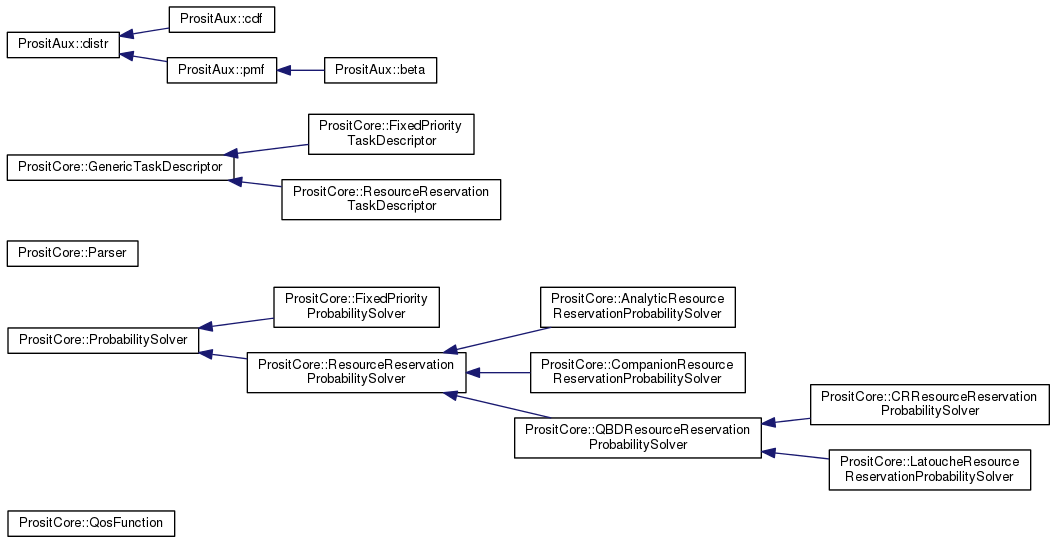
\includegraphics[width=0.9\linewidth]{classdiagram.png}}
  \caption{The PROSIT class diagram generated by Doxygen.}
  \label{automaton}
\end{figure}

\section{Use cases}
% 
% TODO: insert the use case diagram similar to the one in the paper, but slightly modified
%
The most common use case for the PROSIT tools is the analysis problem: the designer is required to enter the parameters to define the task he/she wishes to analyse.\\
Since a it can only be resource reservation task\footnote{The fixed priority type of task is currently under development and it is not available yet.}, the values for the time requirements (the PMF for the computation time and the one for the interarrival time, if the task is aperiodic) and the scheduling parameters \( Q_{i}^s \) and \( T_{i}^s \) must be provided. Thanks to the temporal isolation property defined in Equation \ref{schedCond}, it allows the tool to treat every task on its own if several tasks are passed as inputs to the tool. The distribution functions can be specified inside the task or taken as input from a file.\\
As a result of a tool invocation, all the provided information are analysed and then the solver for the probabilisti deadlines is called. The \emph{apply\_algorithm()} method called by the probability solver object is a pure virtual function\footnote{Pure virtual functions in C++ are used to take advantage of polymorphism. This is essential for providing a unique interface for multiple objects, which implements different versions of the same method, based on the input selection.}; this allows PROSIT to call the right solution strategy selected by the user.

\begin{figure}[H]
  \center{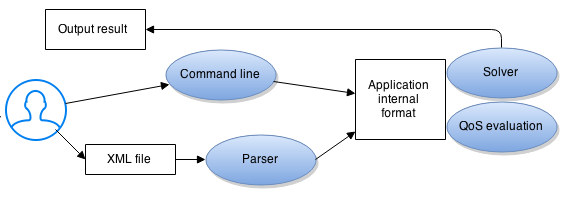
\includegraphics[width=0.7\linewidth]{usecase.png}}
  \caption{The analysis usecase for PROSIT.}
  \label{usecase}
\end{figure}